\documentclass[a4paper, 14pt]{article}
\usepackage[margin=1.6cm]{geometry}
\usepackage[utf8]{inputenc}
\usepackage{minted}
\usepackage[russian]{babel}
\usepackage{amsmath}
\usepackage{graphicx}
\usepackage{changepage}
\usepackage{hyperref}
\usepackage{cases}
\usepackage{tikz-timing}[2017/12/20]
\usepackage{relsize}
\usepackage{booktabs}
\usepackage{gensymb}
\usepackage{multirow}
\usepackage{longtable}
\usepackage{indentfirst}
\usetikzlibrary {arrows.meta}

\hypersetup{
	linkbordercolor = {1 1 1}
}

\usepackage{tikz-timing}[2009/05/15]
\usepackage{multicol}
\usepackage[T2A]{fontenc}
\usepackage{pgfplots}
%\usepackage[left=2.5cm, right=1.5cm, vmargin=2.5cm]{geometry}
\setlength\parindent{0pt} % Удалить отступы из параграфов.

\usepackage{listings}
\usepackage{caption}
\DeclareCaptionFont{white}{\color{white}} % Текст заголовка.
\DeclareCaptionFormat{listing}{\colorbox{gray}{\parbox{\textwidth}{#1#2#3}}}
\captionsetup[lstlisting]{format=listing,labelfont=white,textfont=white}
\renewcommand\labelenumi{\theenumi)}
\setlength\parindent{24pt}



\begin{document}
\lstset{
    language=java,                 % Выбор языка для подсветки (здесь это java).
    basicstyle=\small\sffamily,    % Размер и начертание шрифта для подсветки кода.
    numbers=left,                  % Где поставить нумерацию строк (слева\справа).
    numberstyle=\tiny,             % Размер шрифта для номеров строк.
    stepnumber=1,                  % Размер шага между двумя номерами строк.
    firstnumber=1,
    numberfirstline=true
    numbersep=5pt,                 % Как далеко отстоят номера строк от подсвечиваемого кода.
    backgroundcolor=\color{white}, % Цвет фона подсветки - используем \usepackage{color}.
    showspaces=false,              % Показывать или нет пробелы специальными отступами.
    showstringspaces=false,        % Показывать или нет пробелы в строках.
    showtabs=false,                % Показывать или нет табуляцию в строках.
    frame=single,                  % Рисовать рамку вокруг кода.
    tabsize=2,                     % Размер табуляции по умолчанию равен 2 пробелам.
    captionpos=t,                  % Позиция заголовка вверху [t] или внизу [b].
    breaklines=true,               % Автоматически переносить строки (да\нет).
    breakatwhitespace=false,       % Переносить строки только если есть пробел.
    escapeinside={\%*}{*)}         % Если нужно добавить комментарии в коде.
}

\begin{titlepage}
    \center

    ФЕДЕРАЛЬНОЕ ГОСУДАРСТВЕННОЕ АВТОНОМНОЕ ОБРАЗОВАТЕЛЬНОЕ УЧРЕЖДЕНИЕ ВЫСШЕГО ОБРАЗОВАНИЯ\linebreak
    «Санкт-Петербургский политехнический университет Петра Великого»
    \noindent\rule{500pt}{0.8pt} \\
    \textsc{\Large Институт компьютерных наук и кибербезопасности}\\
    \textsc{\large Высшая школа программной инженерии}\\[1.5cm]

    { \huge \bfseries HIGH-LEVEL DESIGN	\\
    \Large \mdseries АГРЕГАТОР ЦИФРОВЫХ ФИНАНСОВЫХ АКТИВОВ <<ТЕССЕРАКТ>> \\
    \large по дисциплине <<Технологии разработки качественного программного обеспечения>>}\\
    \flushright{
        {\phantom{qwe}}\\[1.0cm]
    }

    \begin{figure}[H]
        \centering
        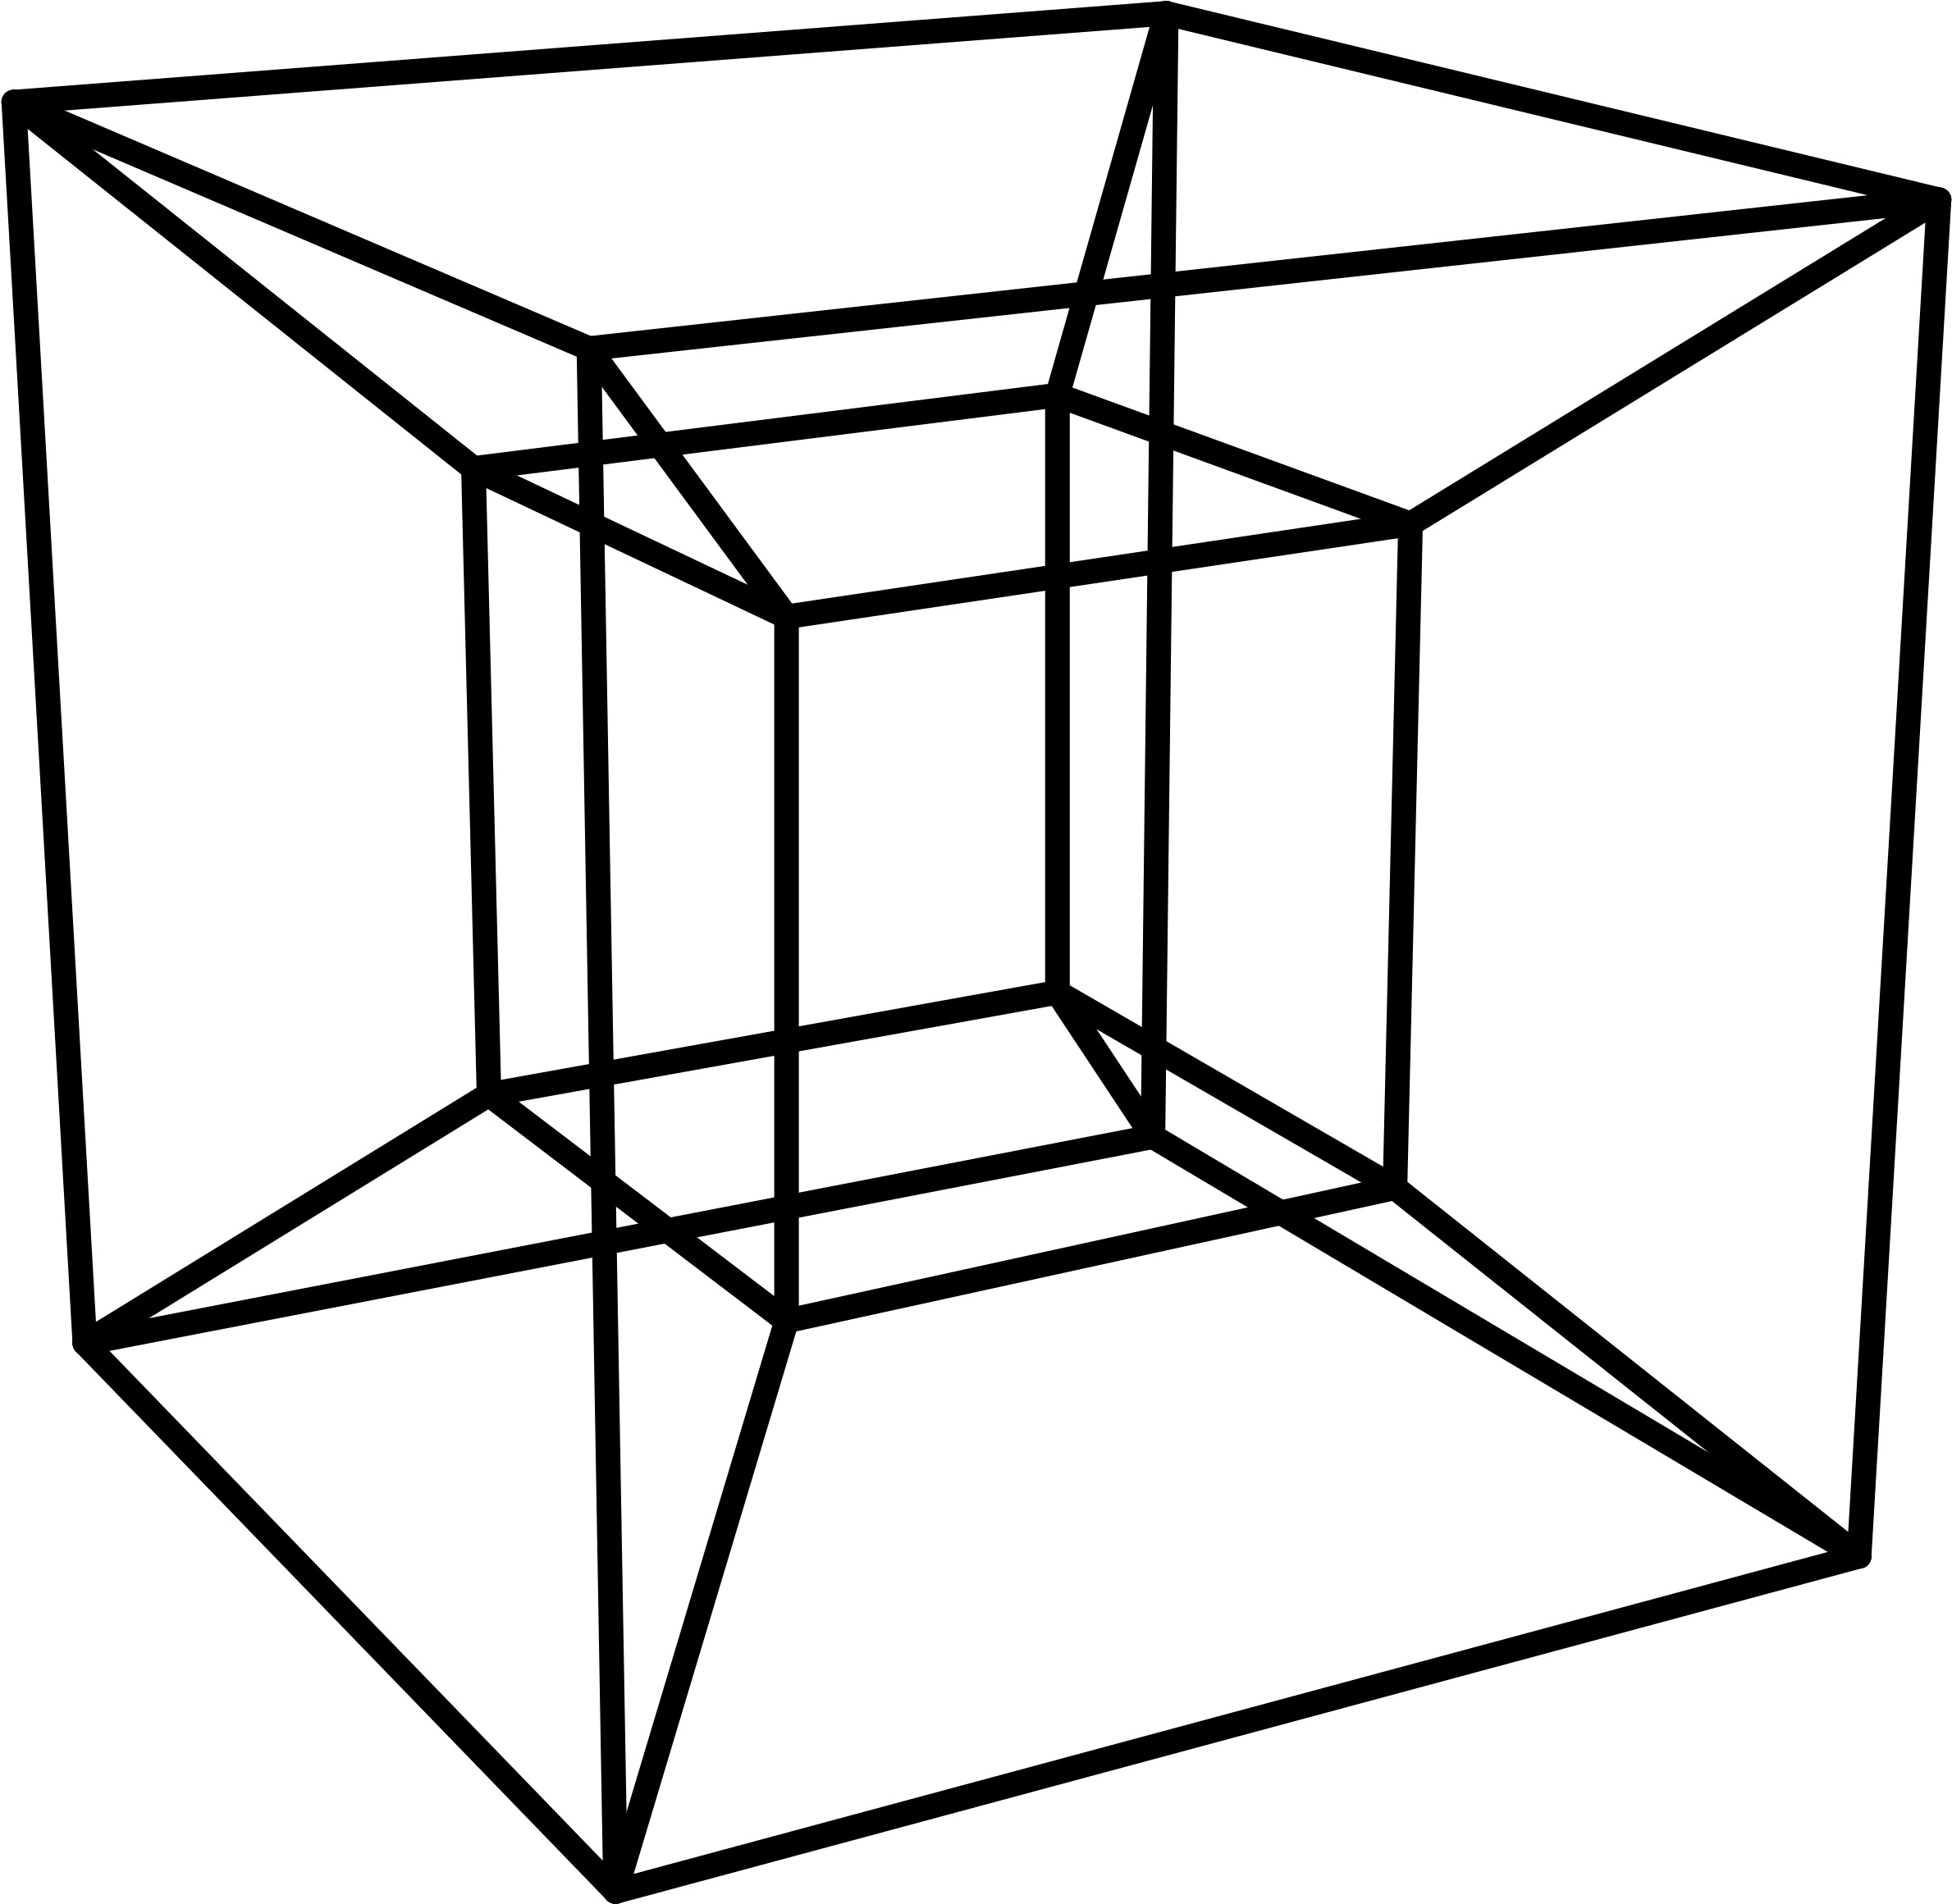
\includegraphics[width=10cm]{resources/1.png}\\[2.0cm]
    \end{figure}

    \begin{multicols}{2}
        \begin{flushright} \large

            {Выполнили студенты группы: 5130904/00104:}\\
            {\phantom{qwe}}\\
            {\phantom{qwe}}\\
            {\phantom{qwe}}\\
            {\phantom{qwe}}\\

            {Преподаватель:\\}

        \end{flushright}
        \begin{flushright}

            {Почернин В. С.}\\
            {Шиляев В. С.}\\
            {Мурзаканов И. М.}\\
            {Разукрантов В. Е.}\\[0.5cm]


            Маслаков А. П.\\

        \end{flushright}
    \end{multicols}

    \flushright{
        {\phantom{qwe}}\\[0.5cm]
    }
    \centering{
        Санкт-Петербург\\
        2023
    }

    \vfill
\end{titlepage}

\Large
\tableofcontents
\newpage
\large

\section{Макет дизайна интерфейса}

\begin{figure}[H]
    \centering
    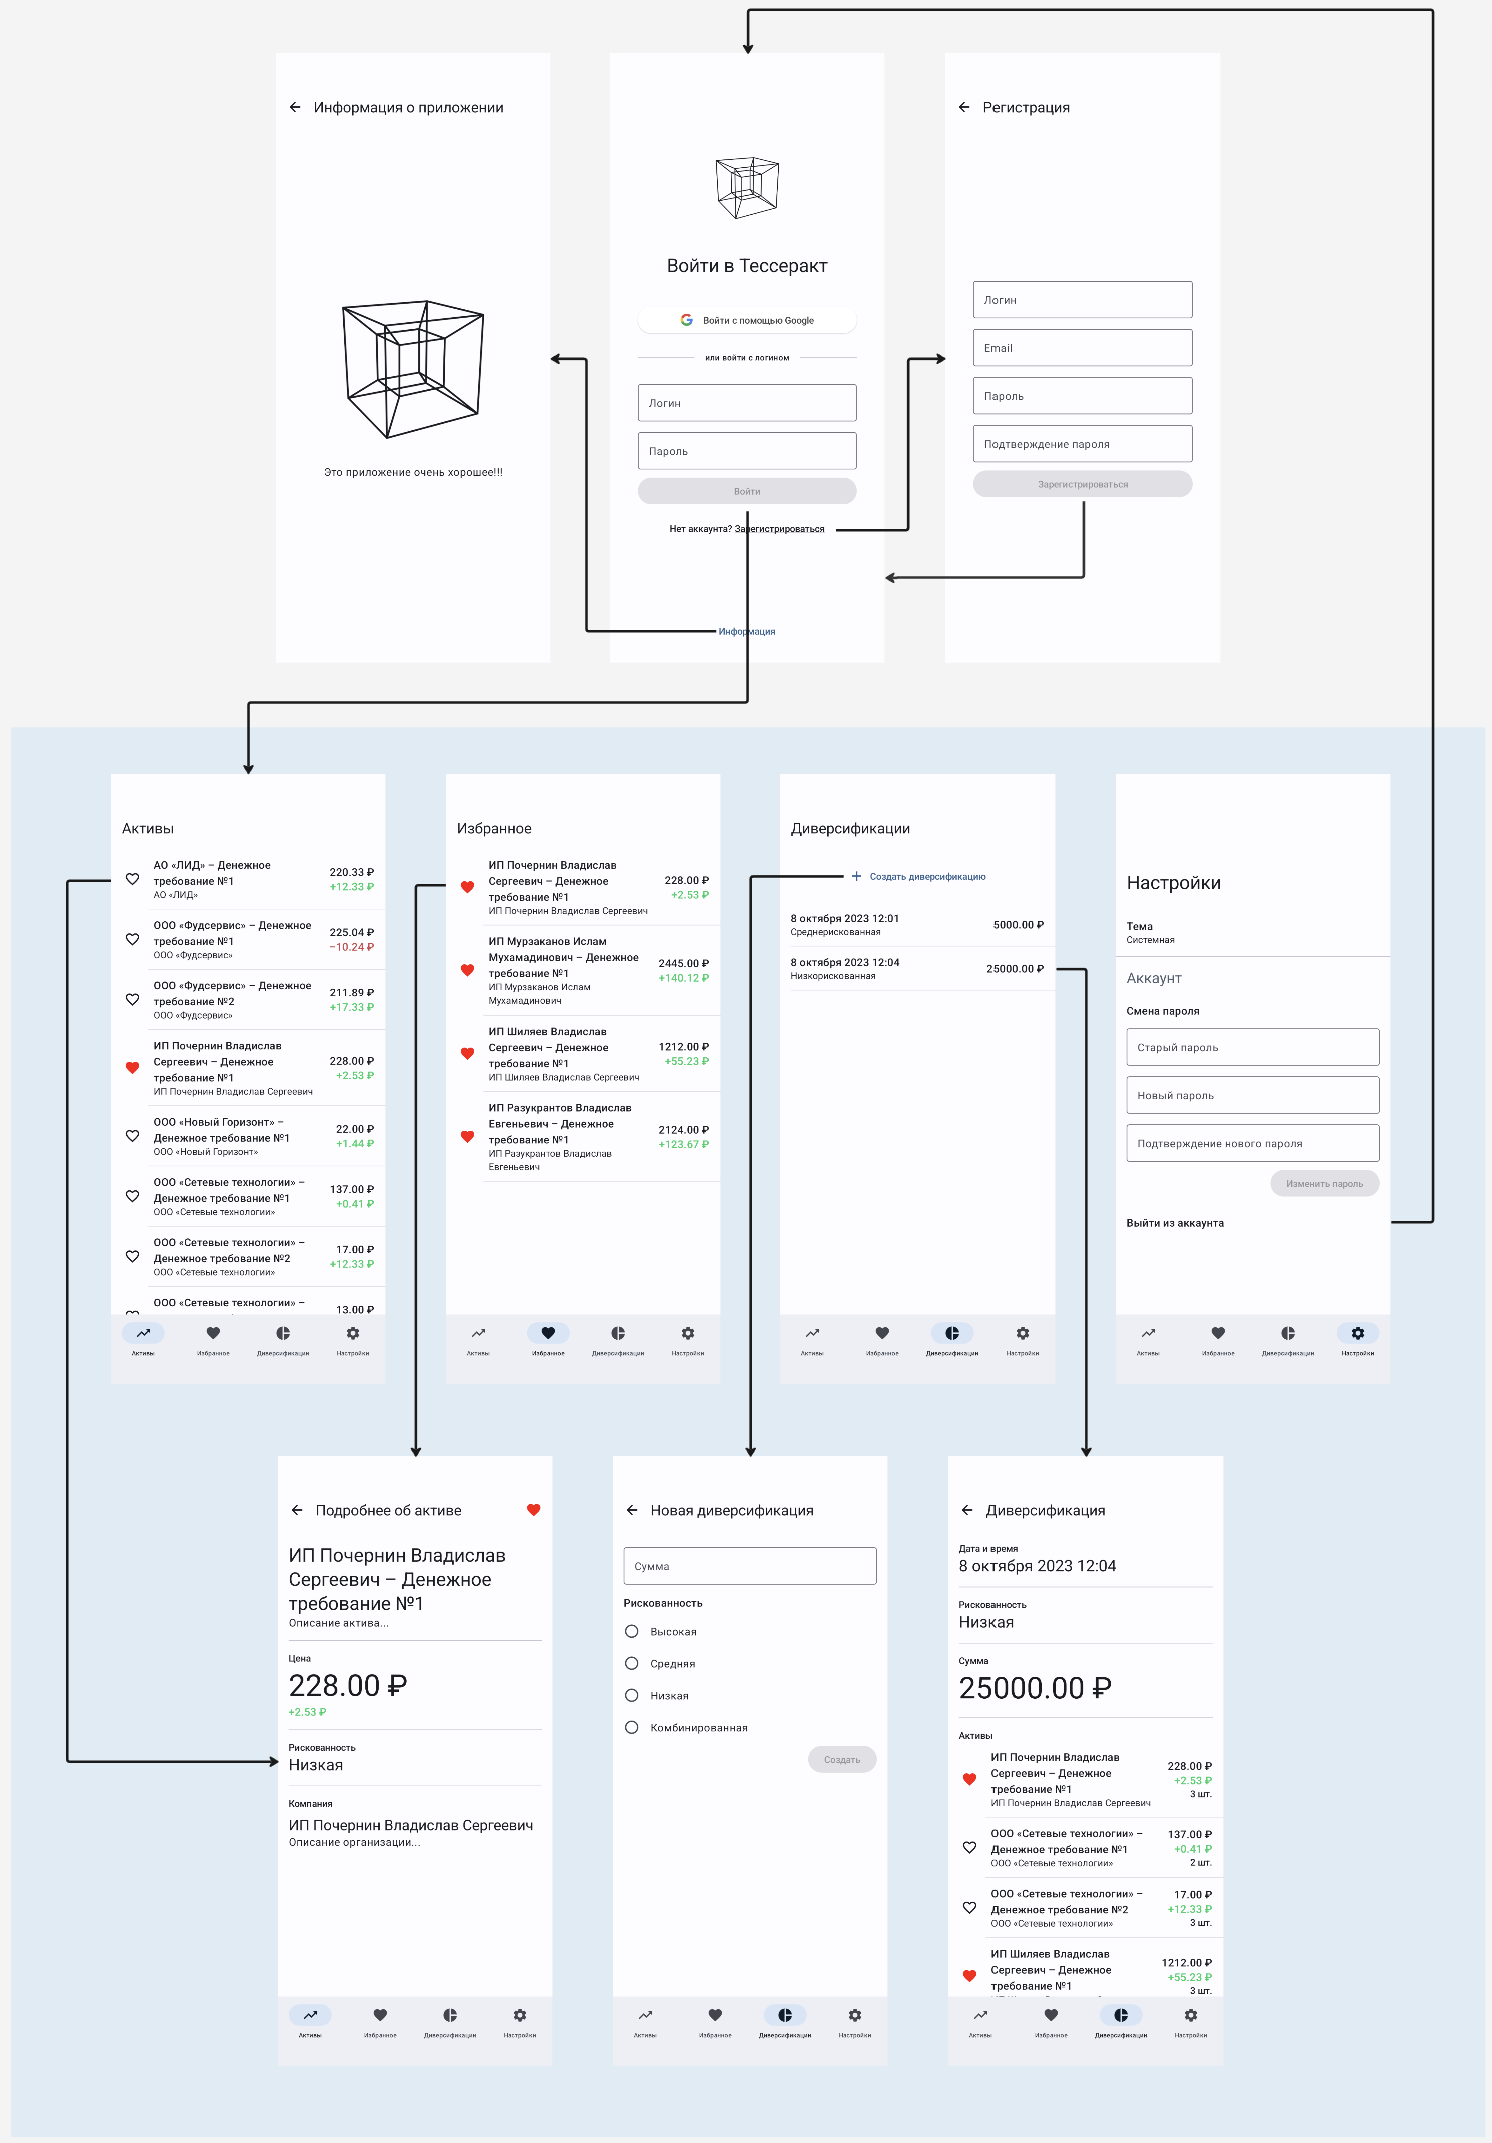
\includegraphics[width=17cm]{resources/3.png}
    \caption{Схема переходов между страницами}
\end{figure}

\subsection{Список страниц}

\begin{enumerate}
    \item Страница входа (LoginPage).
    \item Страница информации (InfoPage).
    \item Страница регистрации (RegistrationPage).
    \item Страница активов (AssetsPage).
    \item Страница конкретного актива (AssetPage).
    \item Страница избранных активов (FavouritesPage).
    \item Страница диверсификаций (DiversificationsPage).
    \item Страница создания диверсификации (DiversificationCreatePage).
    \item Страница конкретной диверсификации (DiversificationPage).
    \item Страница настроек (SettingsPage).
\end{enumerate}

\section{Архитектура приложения}

Клиентская часть приложения реализует паттерны \texttt{Single Activity Application}, а также \texttt{MVVM (Model View ViewModel)}.

Пользователь взаимодействует с UI, написанном на \texttt{Compose}, который в свою очередь получает данные из \texttt{ViewModel} и отправляет действия пользователя во \texttt{ViewModel}.

Клиент же общается с сервером посредством предоставляемого сервером API, внутри которого происходит исполнение бизнес-логики и обращение к БД.

\begin{figure}[H]
    \centering
    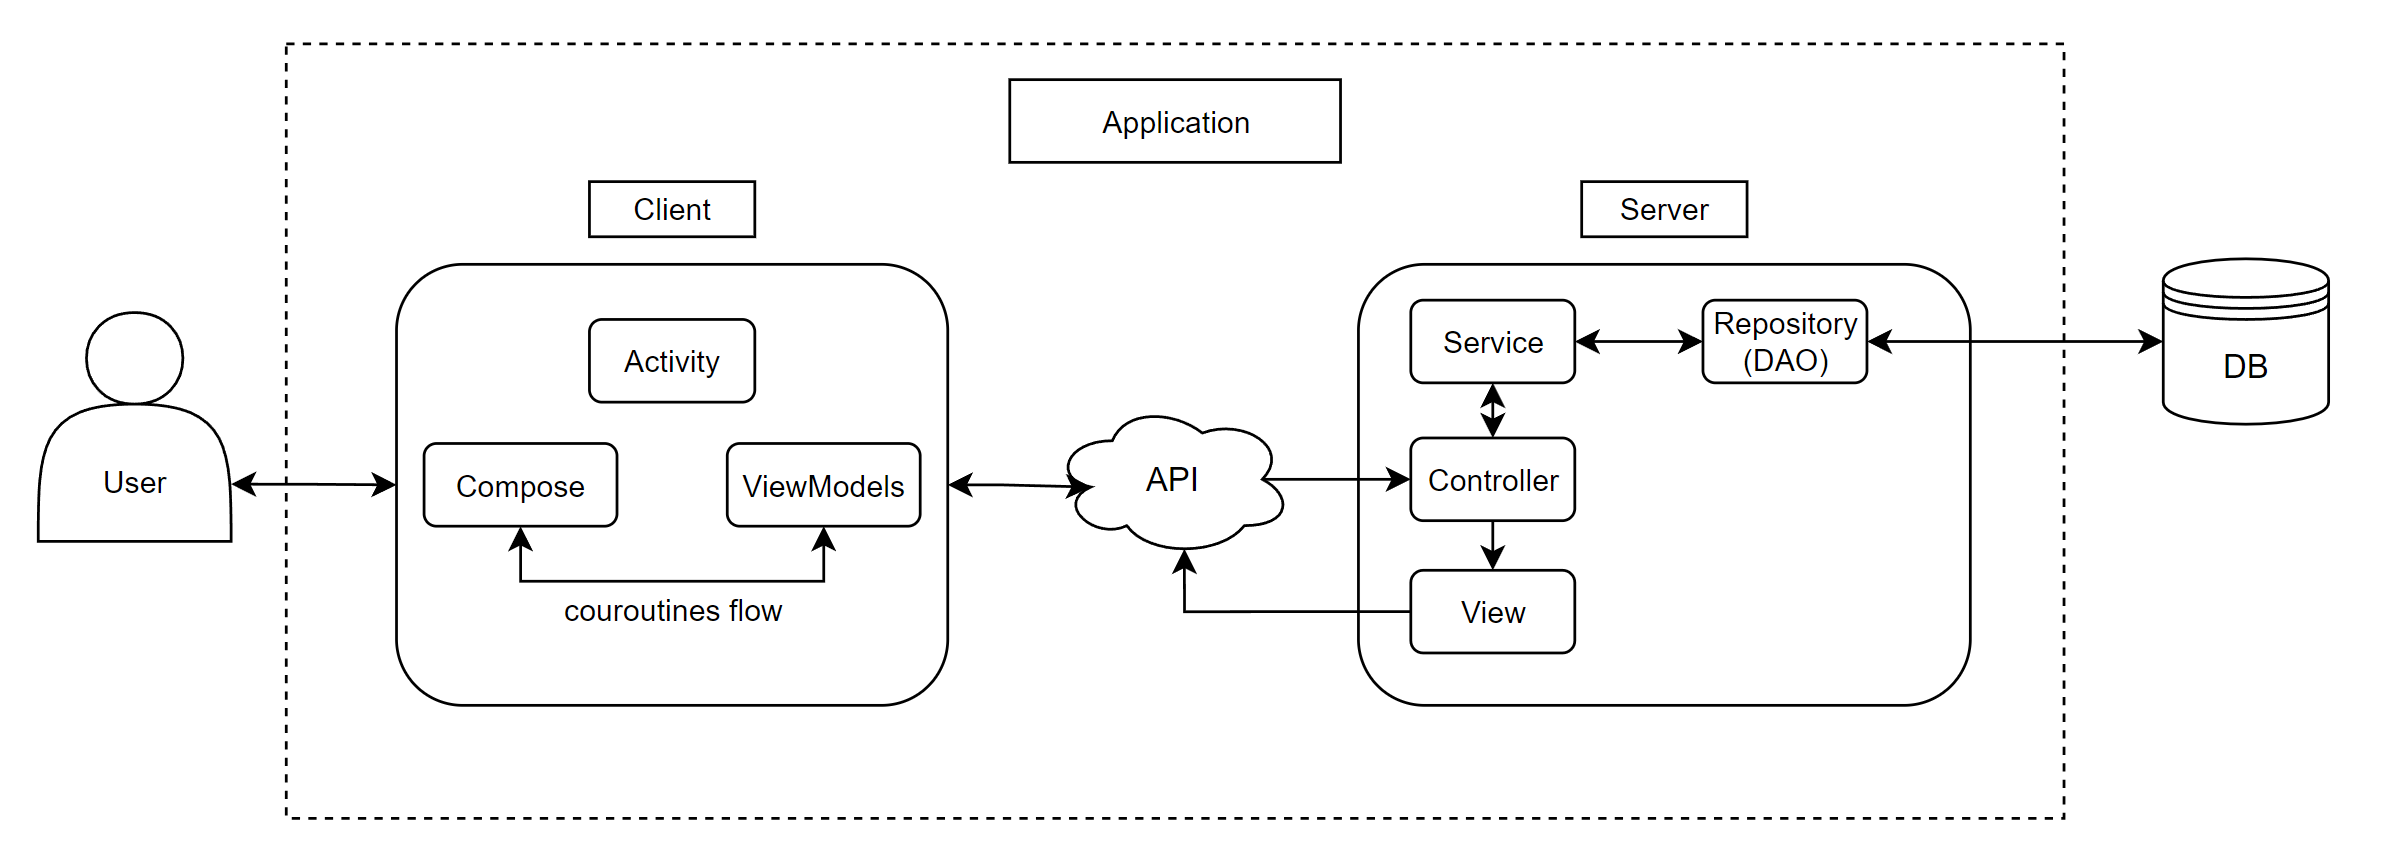
\includegraphics[width=19cm]{resources/2.png}
    \caption{Архитектура приложения}
\end{figure}

\section{Стек технологий}

\subsection{Backend}

\begin{itemize}
    \item \textbf{Java} - язык программирования.
    \item \textbf{Spring} - основной фреймворк.
    \item \textbf{PostgreSQL} - система управления базами данных.
    \item \textbf{Swagger} - инструмент для описания API.
    \item \textbf{Hibernate} - библиотека для задач объектно-реляционного отображения.
\end{itemize}

\subsection{Frontend}

\begin{itemize}
    \item \textbf{Kotlin} - язык программирования.
    \item \textbf{Kotlin Coroutines} - библиотека для асинхронной работы.
    \item \textbf{Ktor} - библиотека для работы с API.
    \item \textbf{Koin} - DI (Dependency Injection) фреймворк.
    \item \textbf{Compose} - библиотека для UI.
\end{itemize}

\section{Диаграмма классов}

\begin{figure}[H]
    \centering
    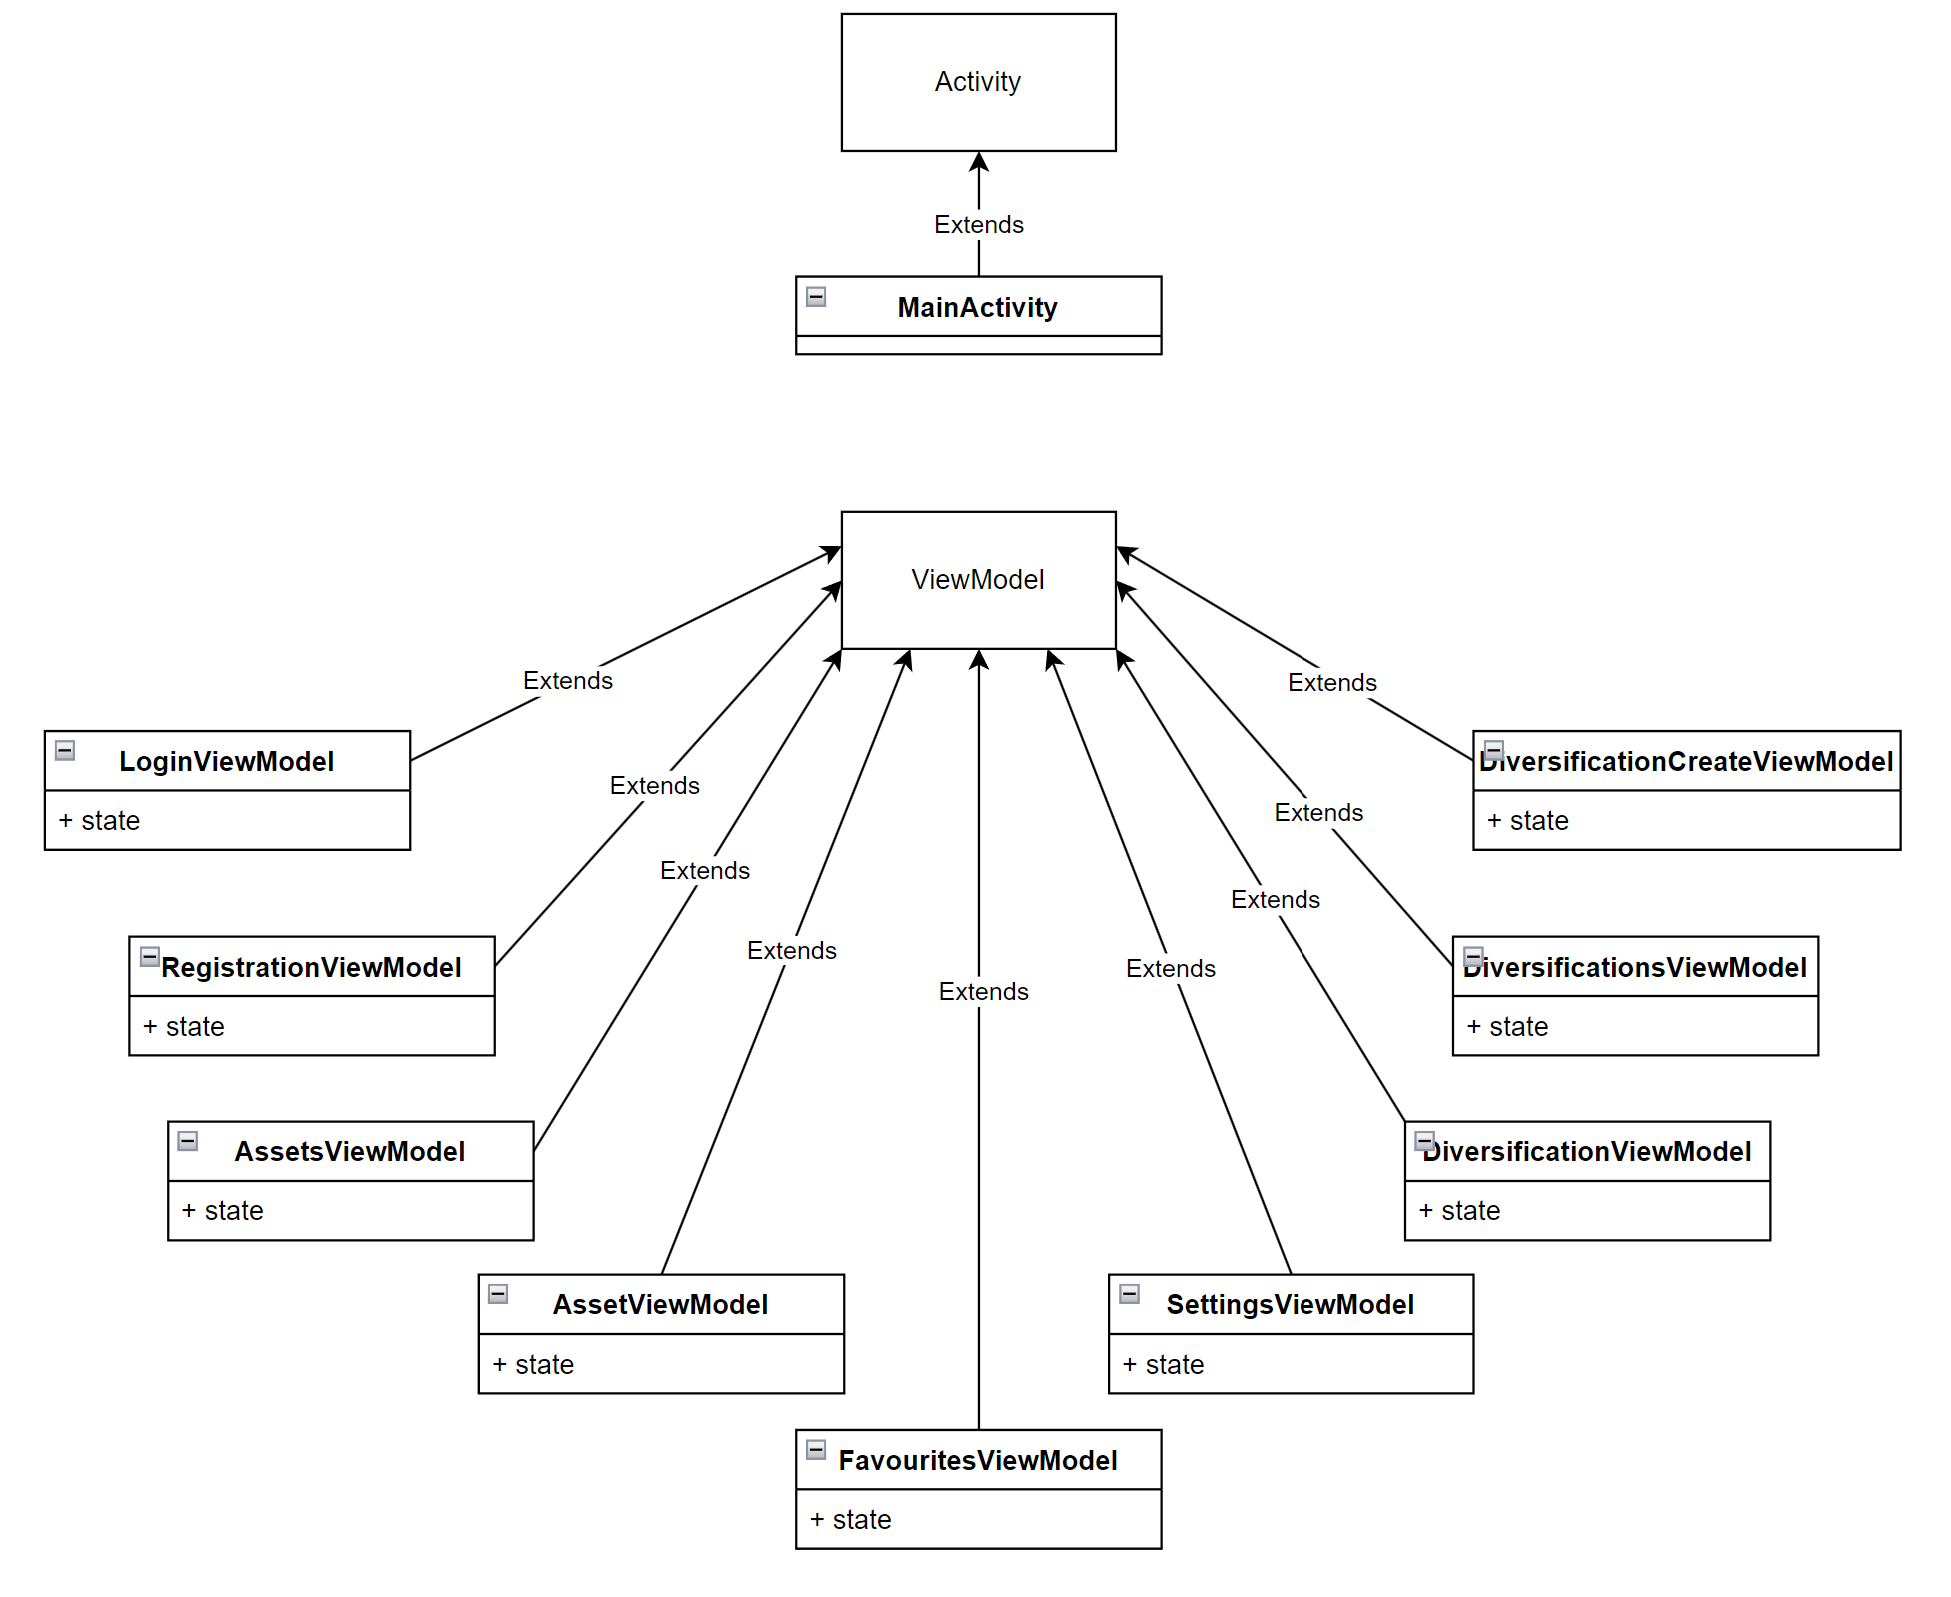
\includegraphics[width=17cm]{resources/15.png}
    \caption{Диаграмма классов}
\end{figure}

\section{Схема базы данных}


\begin{figure}[H]
    \centering
    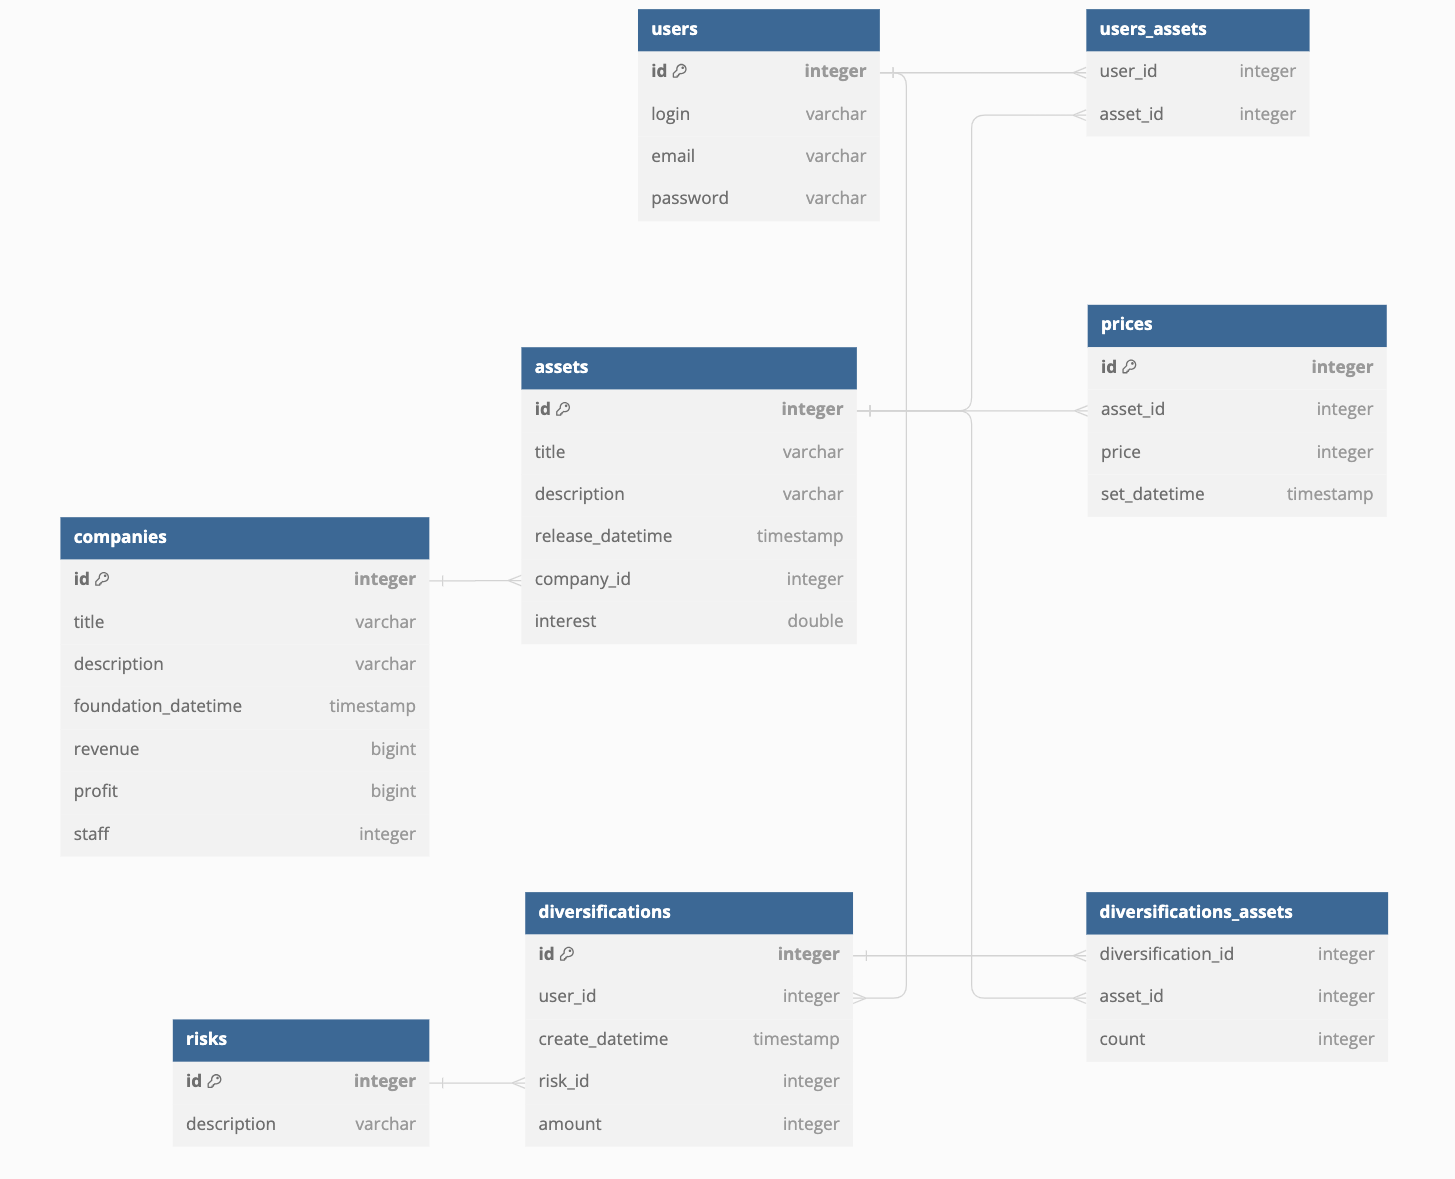
\includegraphics[width=17cm]{resources/14.png}
    \caption{Схема базы данных}
\end{figure}

\section{API}

\subsection{Аутентификация через логин и пароль}

\begin{itemize}
    \item Тип запроса: GET.
    \item Путь запроса: /login.
    \item Входные параметры запроса: логин, пароль.
    \item Выходные параметры запроса: токен.
\end{itemize}

\subsection{Аутентификация через Google OAuth}

\begin{itemize}
    \item Тип запроса: GET.
    \item Путь запроса: /loginByGoogle.
    \item Входные параметры запроса: токен.
    \item Выходные параметры запроса: ???.
\end{itemize}

\subsection{Регистрация пользователя}

\begin{itemize}
    \item Тип запроса: POST.
    \item Путь запроса: /register.
    \item Входные параметры запроса: логин, пароль, email.
    \item Выходные параметры запроса: -.
\end{itemize}

\subsection{Получить список всех активов}

\begin{itemize}
    \item Тип запроса: GET.
    \item Путь запроса: /assets/{id}.
    \item Входные параметры запроса: id последнего загруженного актива.
    \item Выходные параметры запроса: список активов (название актива, название компании, стоимость, изменение стоимости, статус избранного).
\end{itemize}

\subsection{Добавить актив в избранное}

\begin{itemize}
    \item Тип запроса: POST.
    \item Путь запроса: /addFavourite/{id}.
    \item Входные параметры запроса: id добавляемого в избранное актива.
    \item Выходные параметры запроса: -.
\end{itemize}

\subsection{Удалить актив из избранного}

\begin{itemize}
    \item Тип запроса: POST.
    \item Путь запроса: /removeFavourite/{id}.
    \item Входные параметры запроса: id удаляемого из избранного актива.
    \item Выходные параметры запроса: -.
\end{itemize}

\subsection{Получить информацию о конкретном активе}

\begin{itemize}
    \item Тип запроса: GET.
    \item Путь запроса: /asset/{id}.
    \item Входные параметры запроса: id актива.
    \item Выходные параметры запроса: название, описание актива, стоимость, изменение стоимости, рискованность, компания, описание компании, статус избранного.
\end{itemize}

\subsection{Получить список избранных активов}

\begin{itemize}
    \item Тип запроса: GET.
    \item Путь запроса: /favouritesAssets.
    \item Входные параметры запроса: id последнего загруженного избранного актива.
    \item Выходные параметры запроса: список избранных активов (название актива, название компании, стоимость, изменение стоимости, статус избранного).
\end{itemize}

\subsection{Получить список диверсификаций}

\begin{itemize}
    \item Тип запроса: GET.
    \item Путь запроса: /diversifications/{id}.
    \item Входные параметры запроса: id последней загруженной диверсификации.
    \item Выходные параметры запроса: список диверсификаций (дата и время создания, степень рискованности, сумма).
\end{itemize}

\subsection{Создать диверсификацию}

\begin{itemize}
    \item Тип запроса: POST.
    \item Путь запроса: /createDiversification.
    \item Входные параметры запроса: сумма, степень рискованности.
    \item Выходные параметры запроса: -.
\end{itemize}

\subsection{Получить информацию о конкретной диверсификации}

\begin{itemize}
    \item Тип запроса: GET.
    \item Путь запроса: /diversification/{id}.
    \item Входные параметры запроса: id диверсификации.
    \item Выходные параметры запроса: дата и время создания, степень рискованности, сумма, список активов (название актива, название компании, общая стоимость данного вида актива (старая), изменение стоимости (по отношению к текущей общей стоимости данного вида актива) ???, количество активов данного вида).
\end{itemize}

\subsection{Изменить пароль}

\begin{itemize}
    \item Тип запроса: PUT.
    \item Путь запроса: /changePassword.
    \item Входные параметры запроса: старый пароль, новый пароль.
    \item Выходные параметры запроса: -.
\end{itemize}

\newpage
\section{Приложение 1: список страниц (экранов)}

\begin{figure}[H]
    \centering
    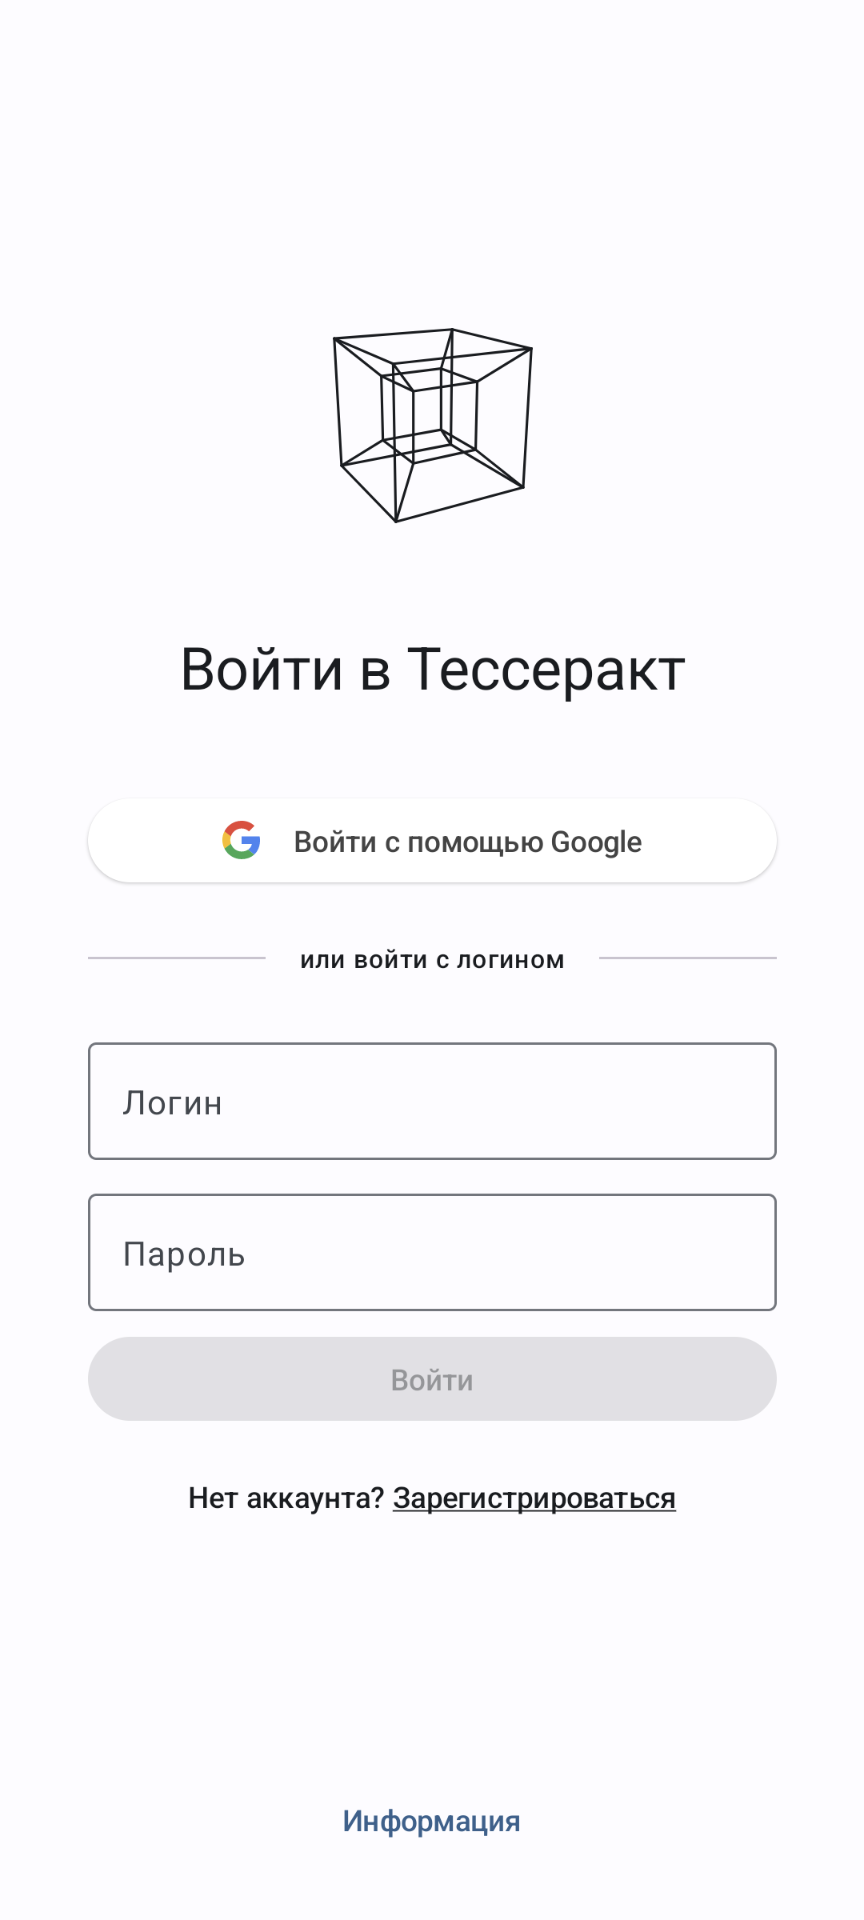
\includegraphics[width=5cm]{resources/4.png}
    \caption{Страница входа (LoginPage)}
\end{figure}

\begin{figure}[H]
    \centering
    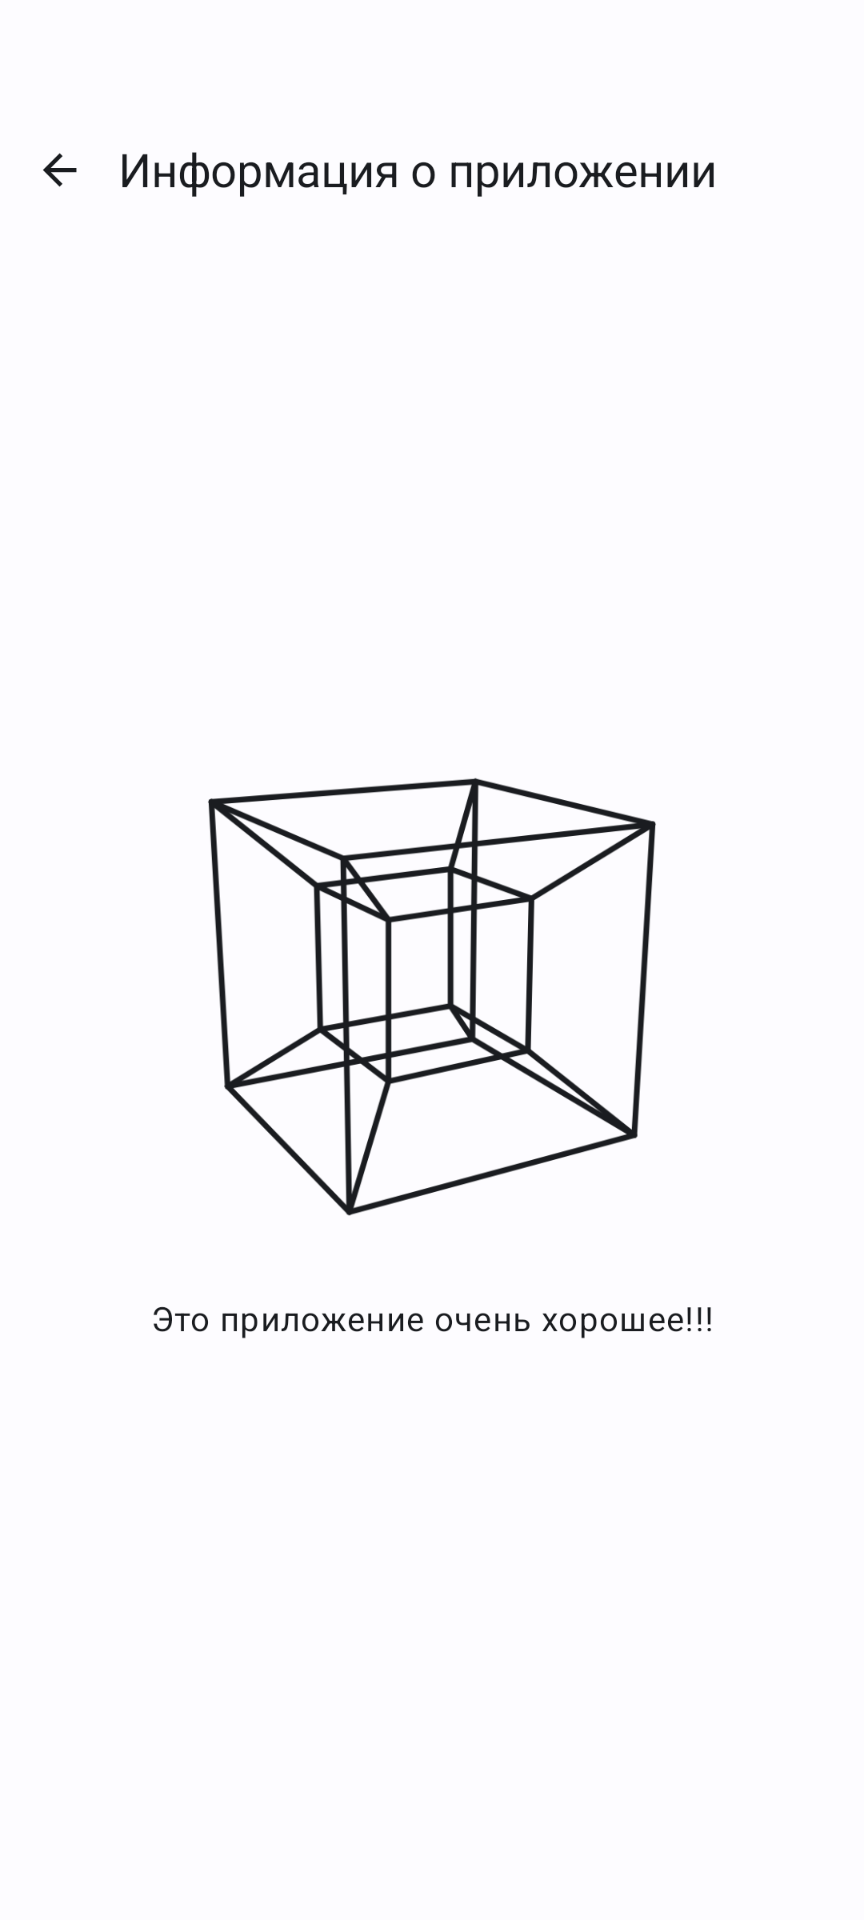
\includegraphics[width=5cm]{resources/5.png}
    \caption{Страница информации (InfoPage)}
\end{figure}

\begin{figure}[H]
    \centering
    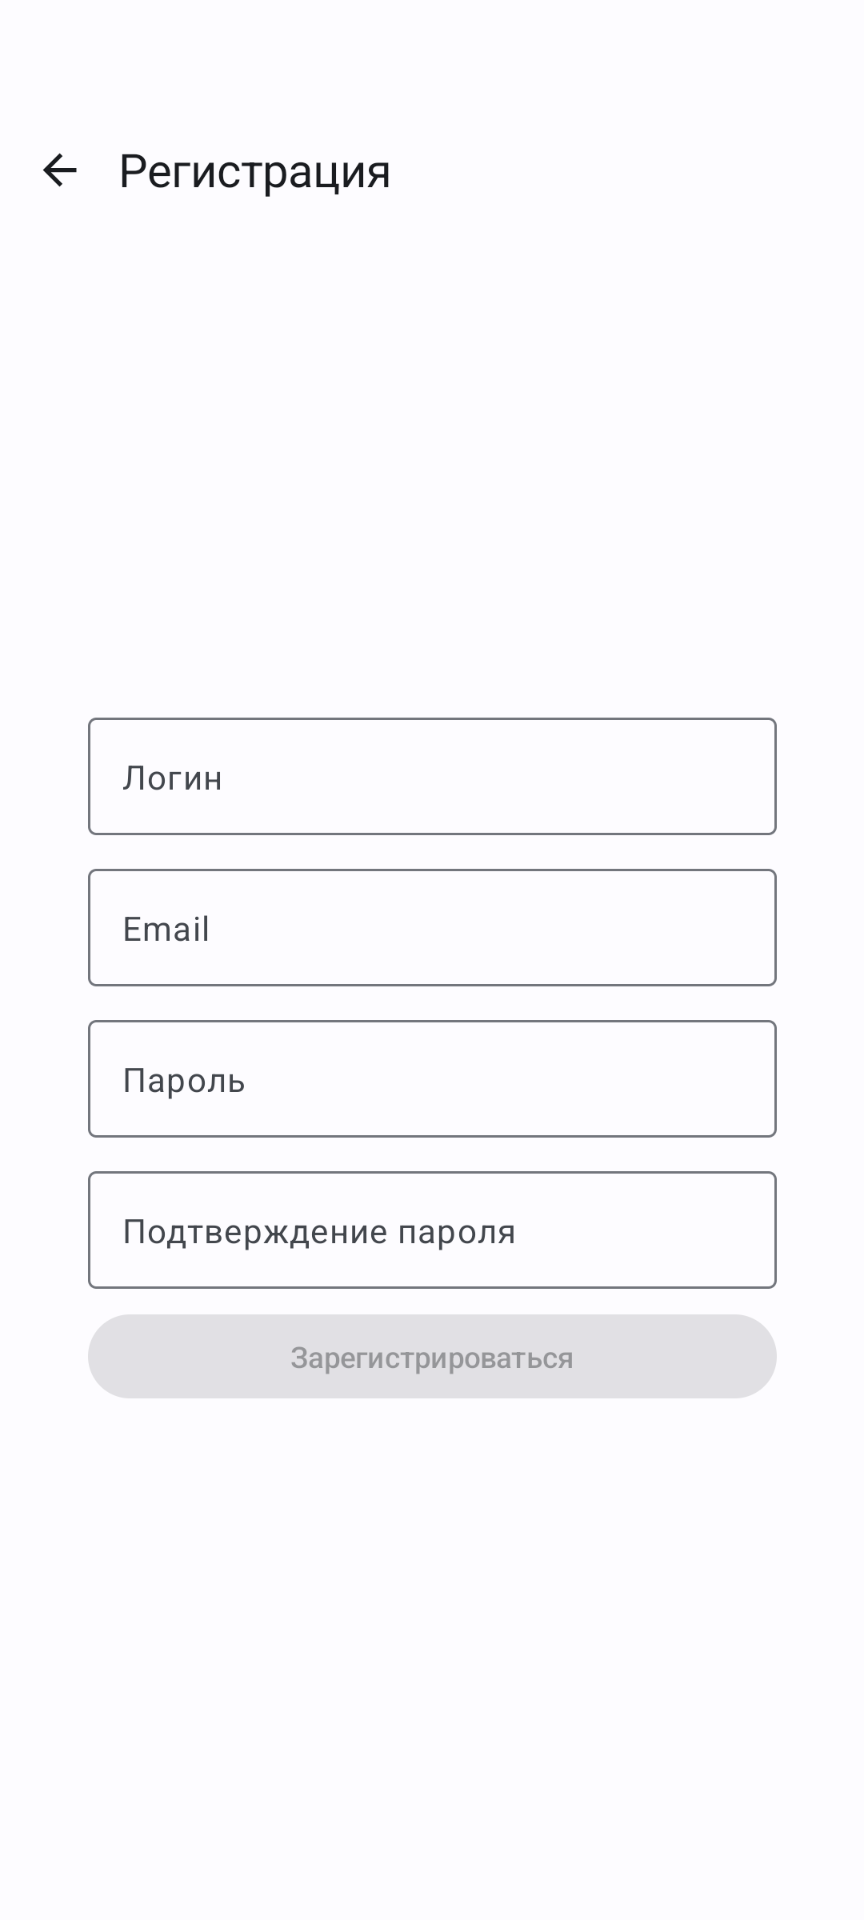
\includegraphics[width=5cm]{resources/6.png}
    \caption{Страница регистрации (RegistrationPage)}
\end{figure}

\begin{figure}[H]
    \centering
    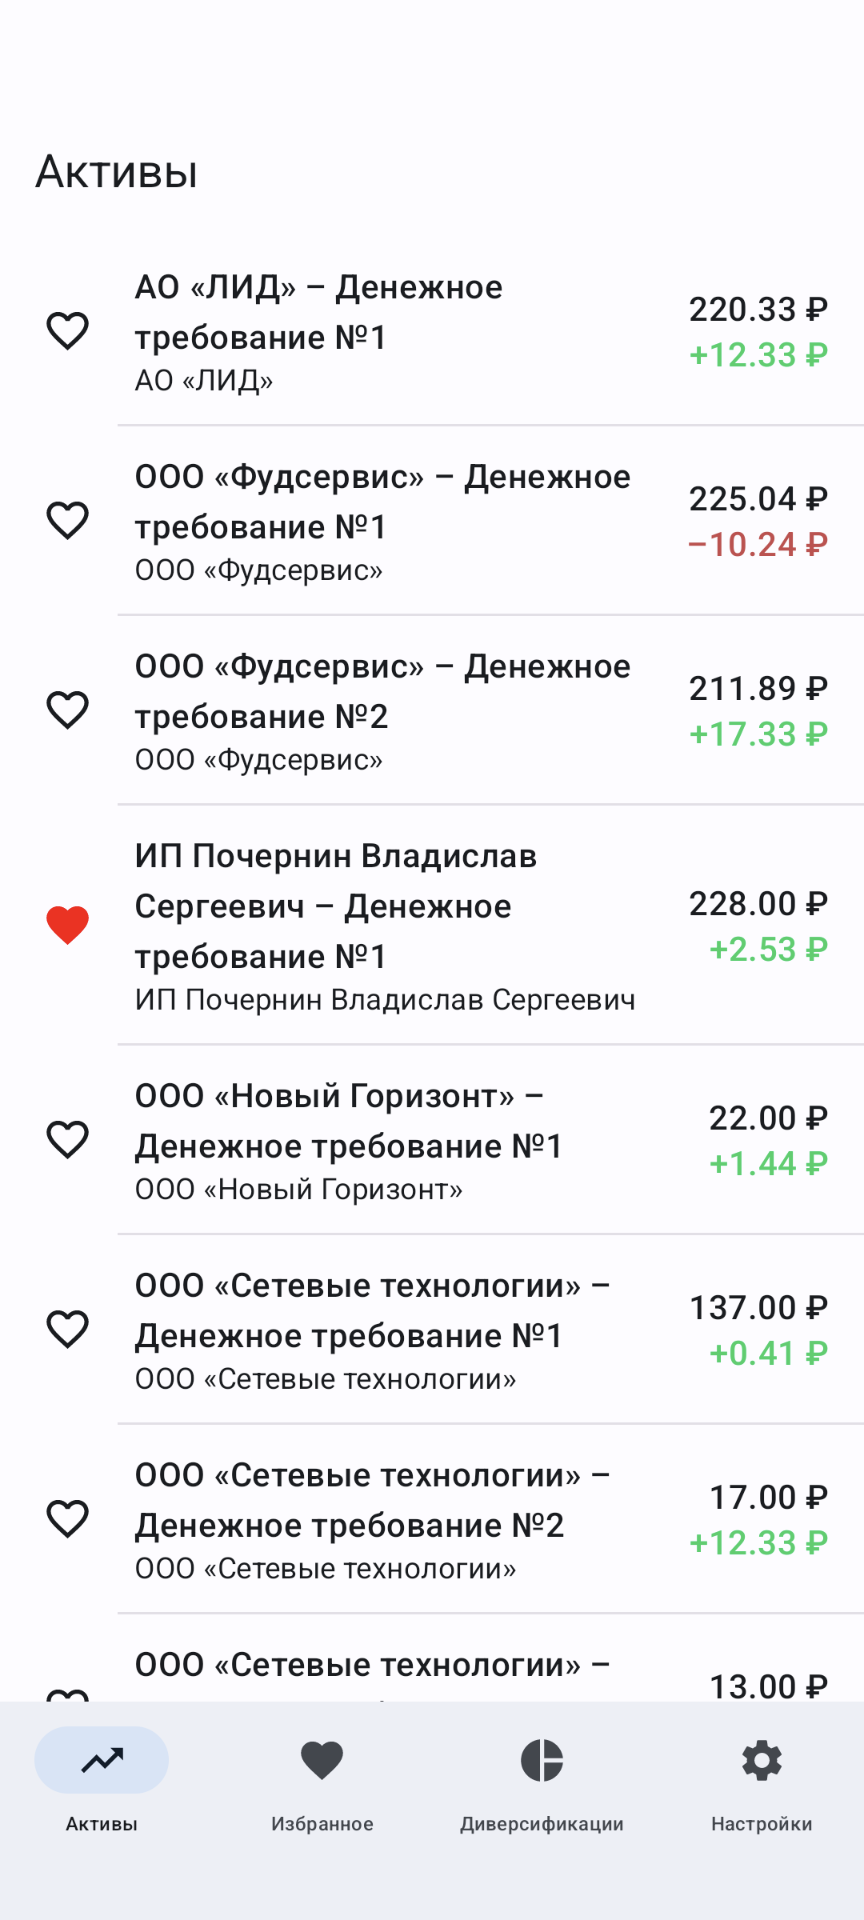
\includegraphics[width=5cm]{resources/7.png}
    \caption{Страница активов (AssetsPage)}
\end{figure}

\begin{figure}[H]
    \centering
    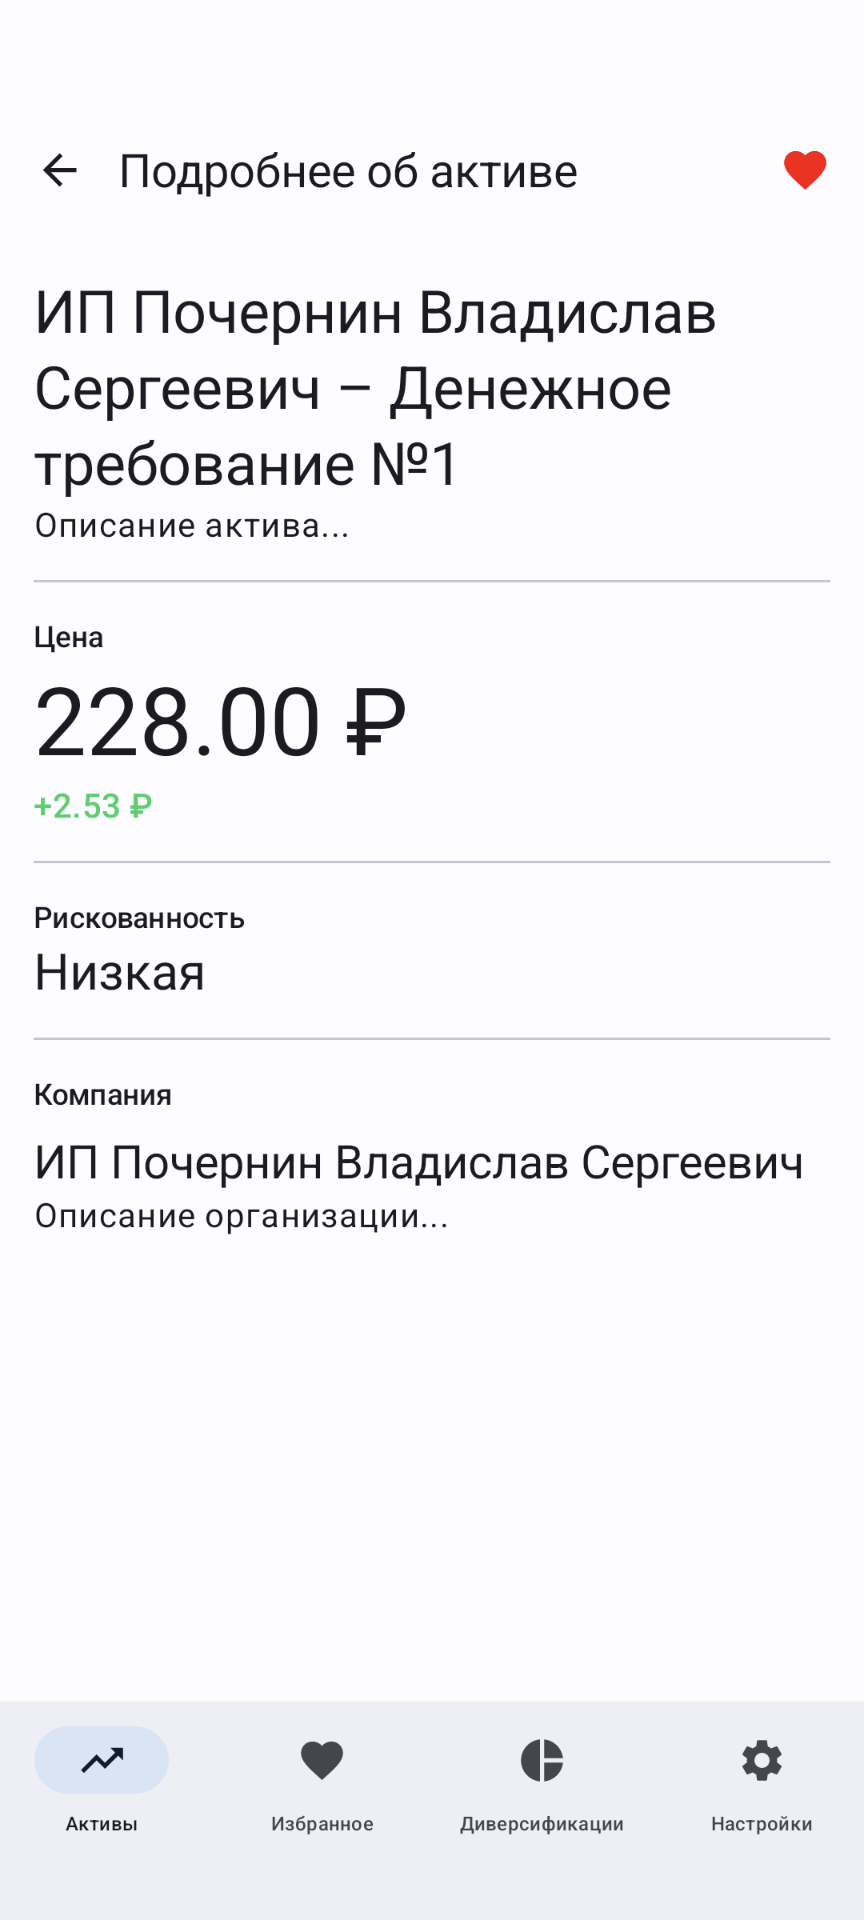
\includegraphics[width=5cm]{resources/8.png}
    \caption{Страница конкретного актива (AssetPage)}
\end{figure}

\begin{figure}[H]
    \centering
    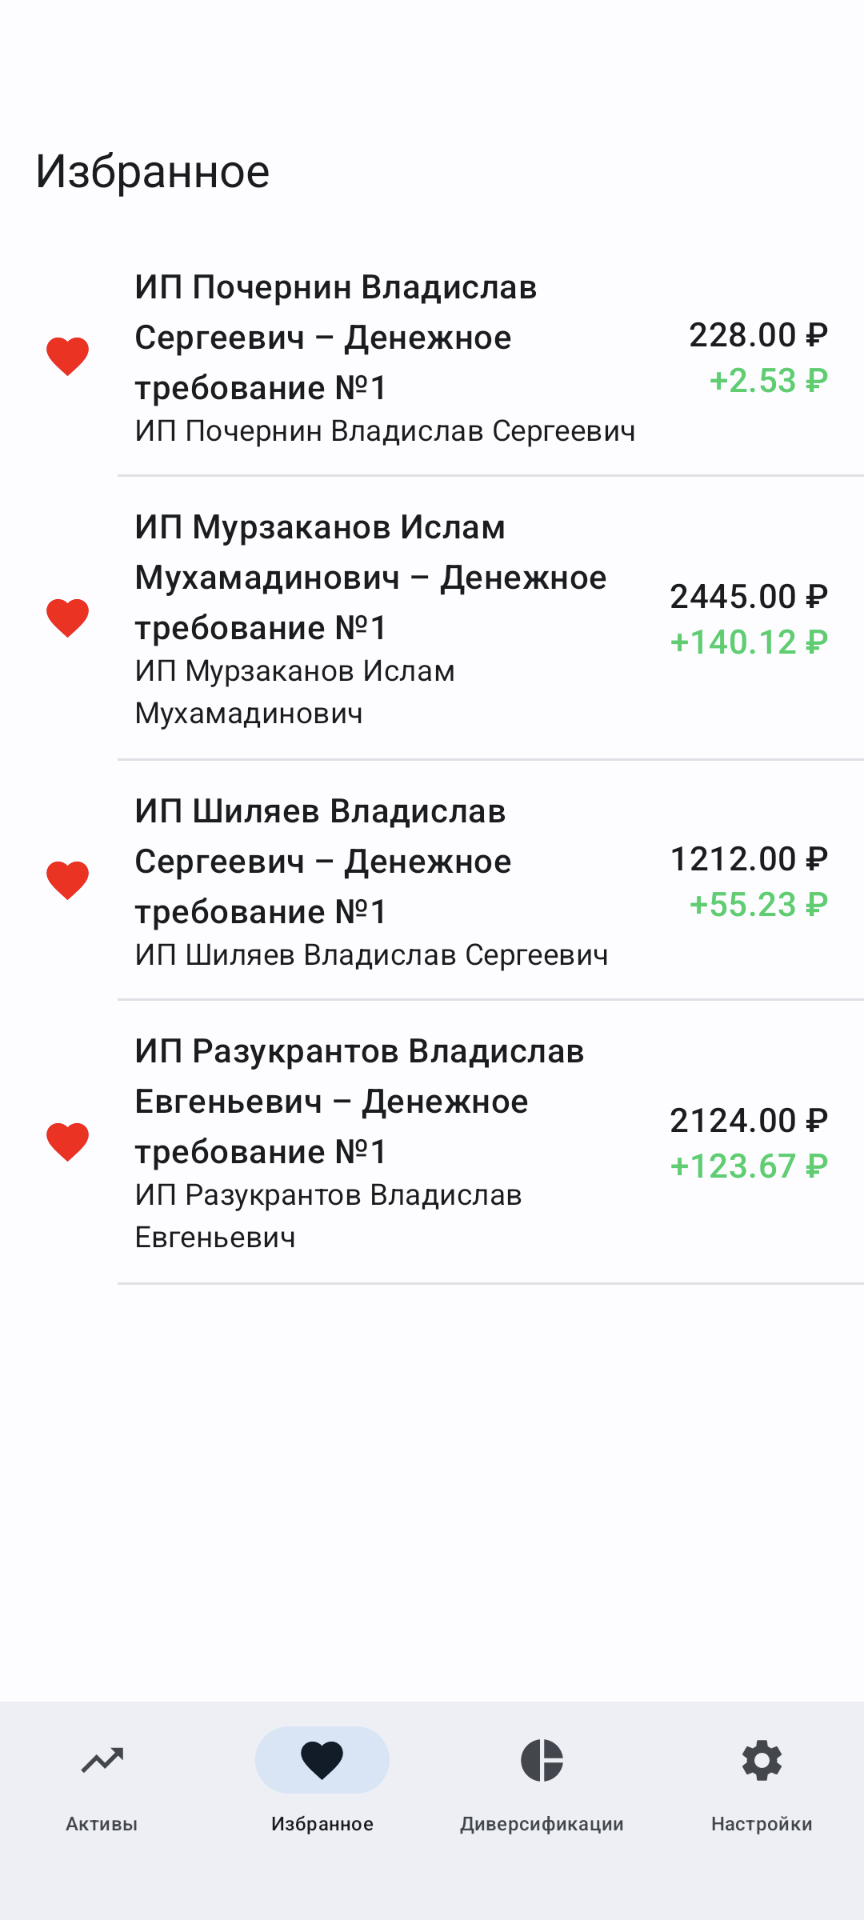
\includegraphics[width=5cm]{resources/9.png}
    \caption{Страница избранных активов (FavouritesPage)}
\end{figure}

\begin{figure}[H]
    \centering
    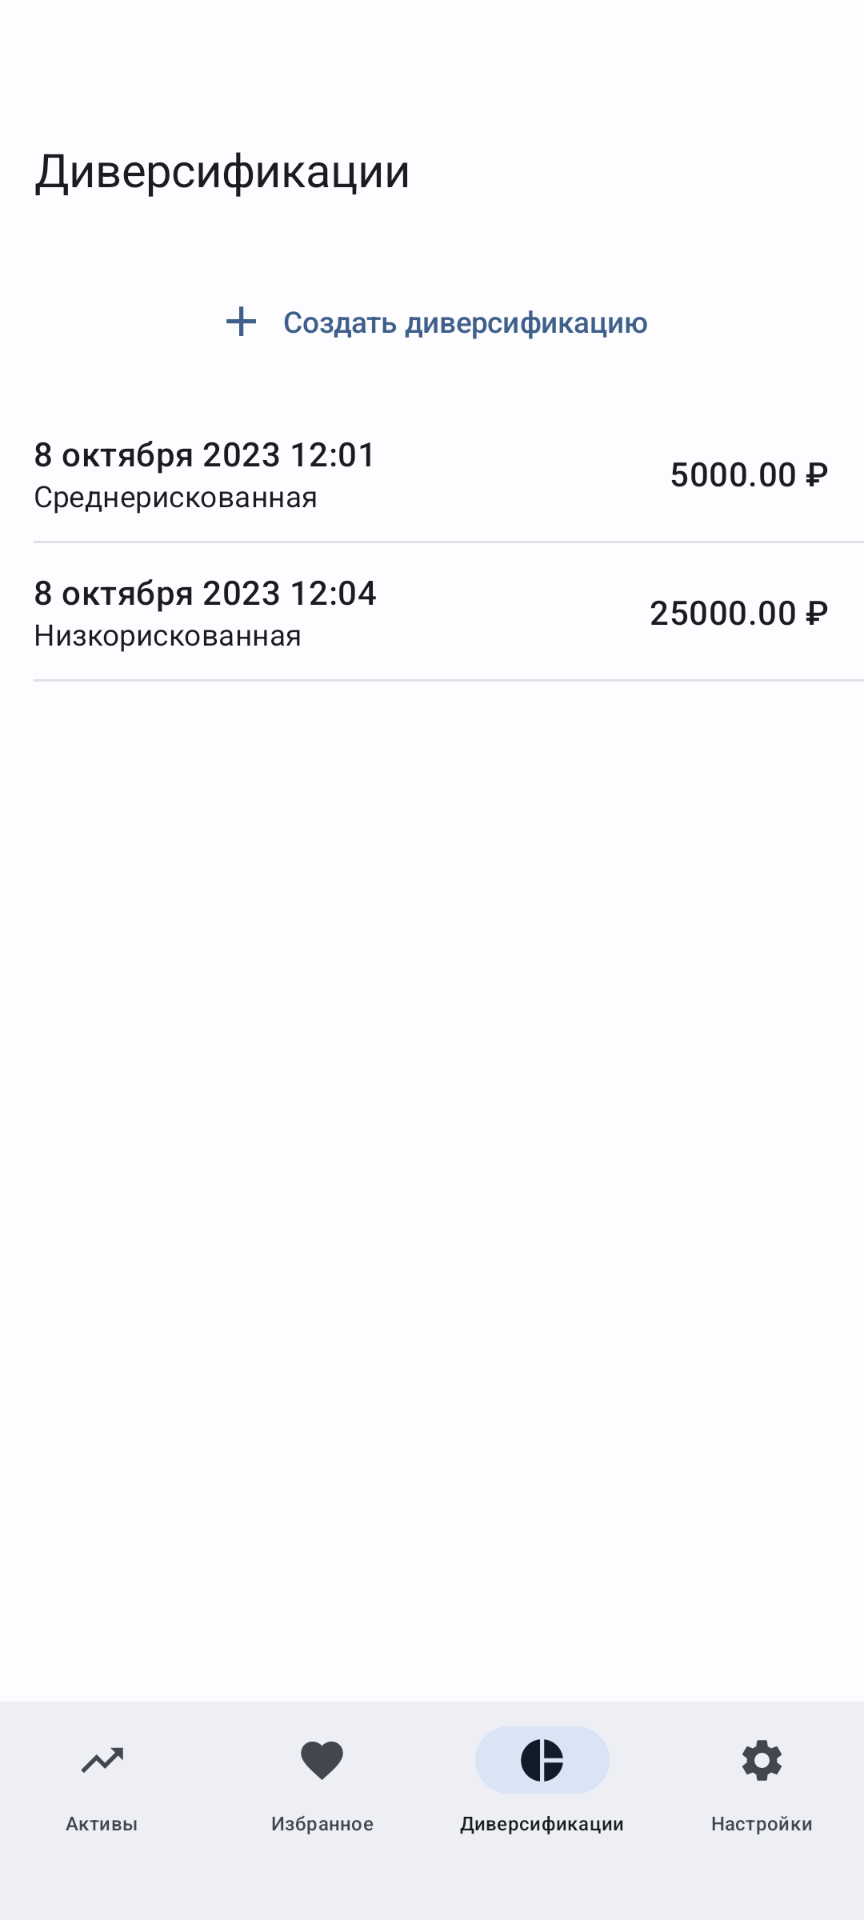
\includegraphics[width=5cm]{resources/10.png}
    \caption{Страница диверсификаций (DiversificationsPage)}
\end{figure}

\begin{figure}[H]
    \centering
    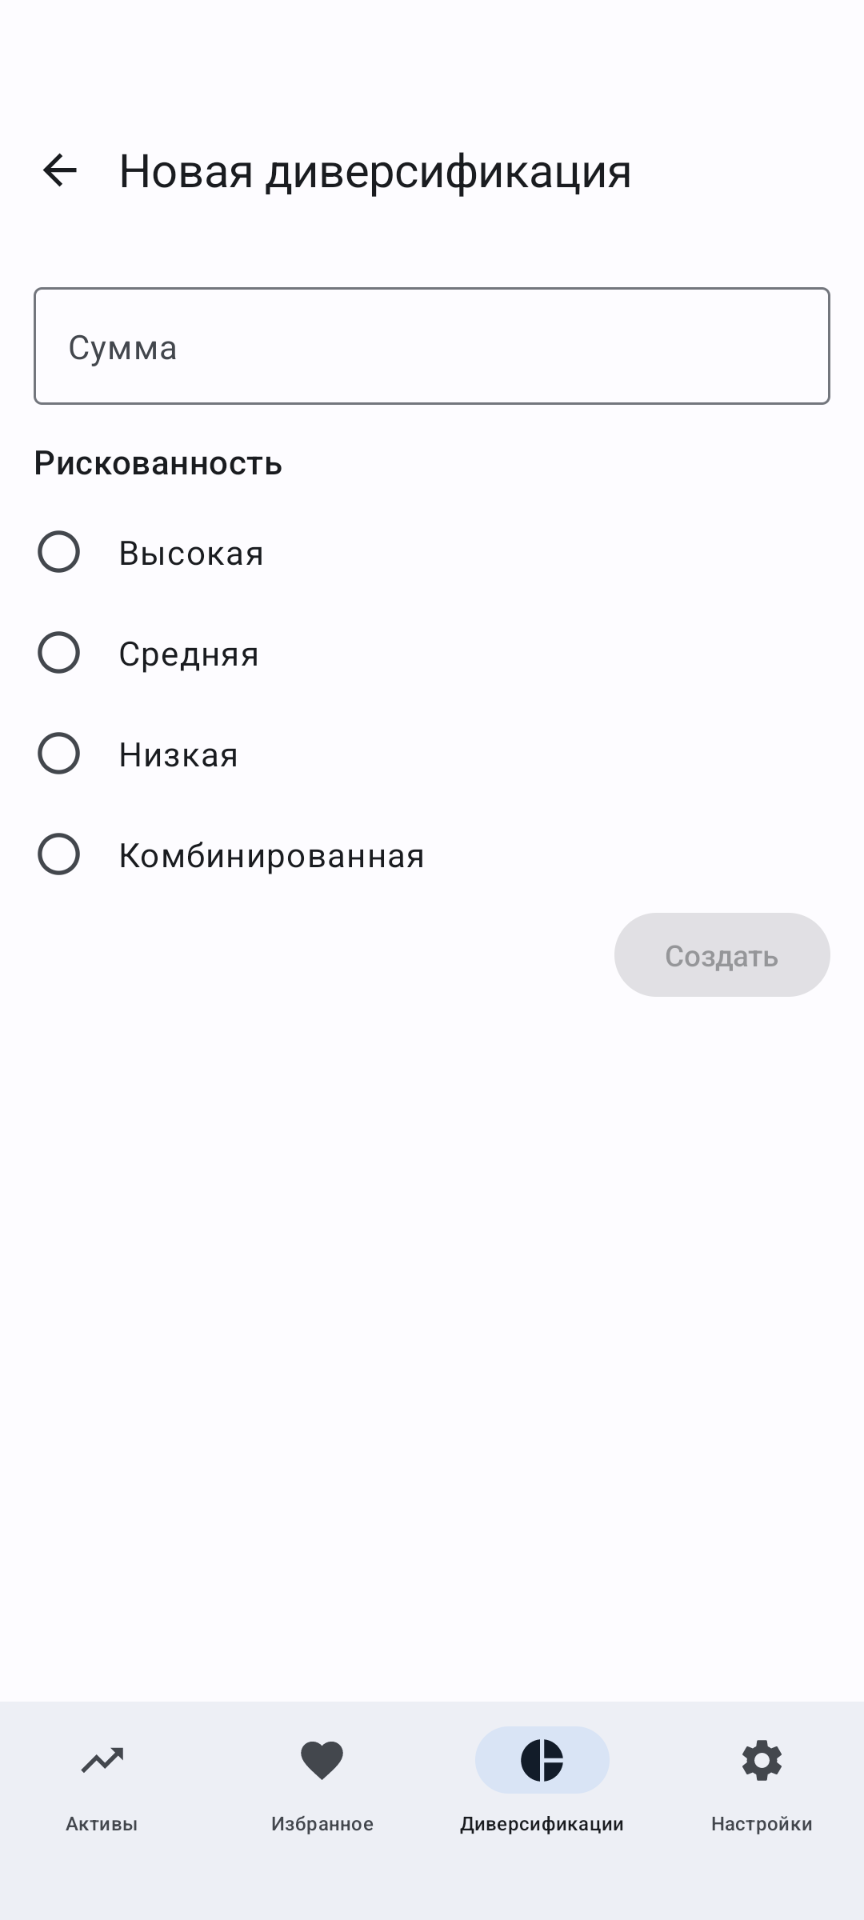
\includegraphics[width=5cm]{resources/11.png}
    \caption{Страница создания диверсификации (DiversificationCreatePage)}
\end{figure}

\begin{figure}[H]
    \centering
    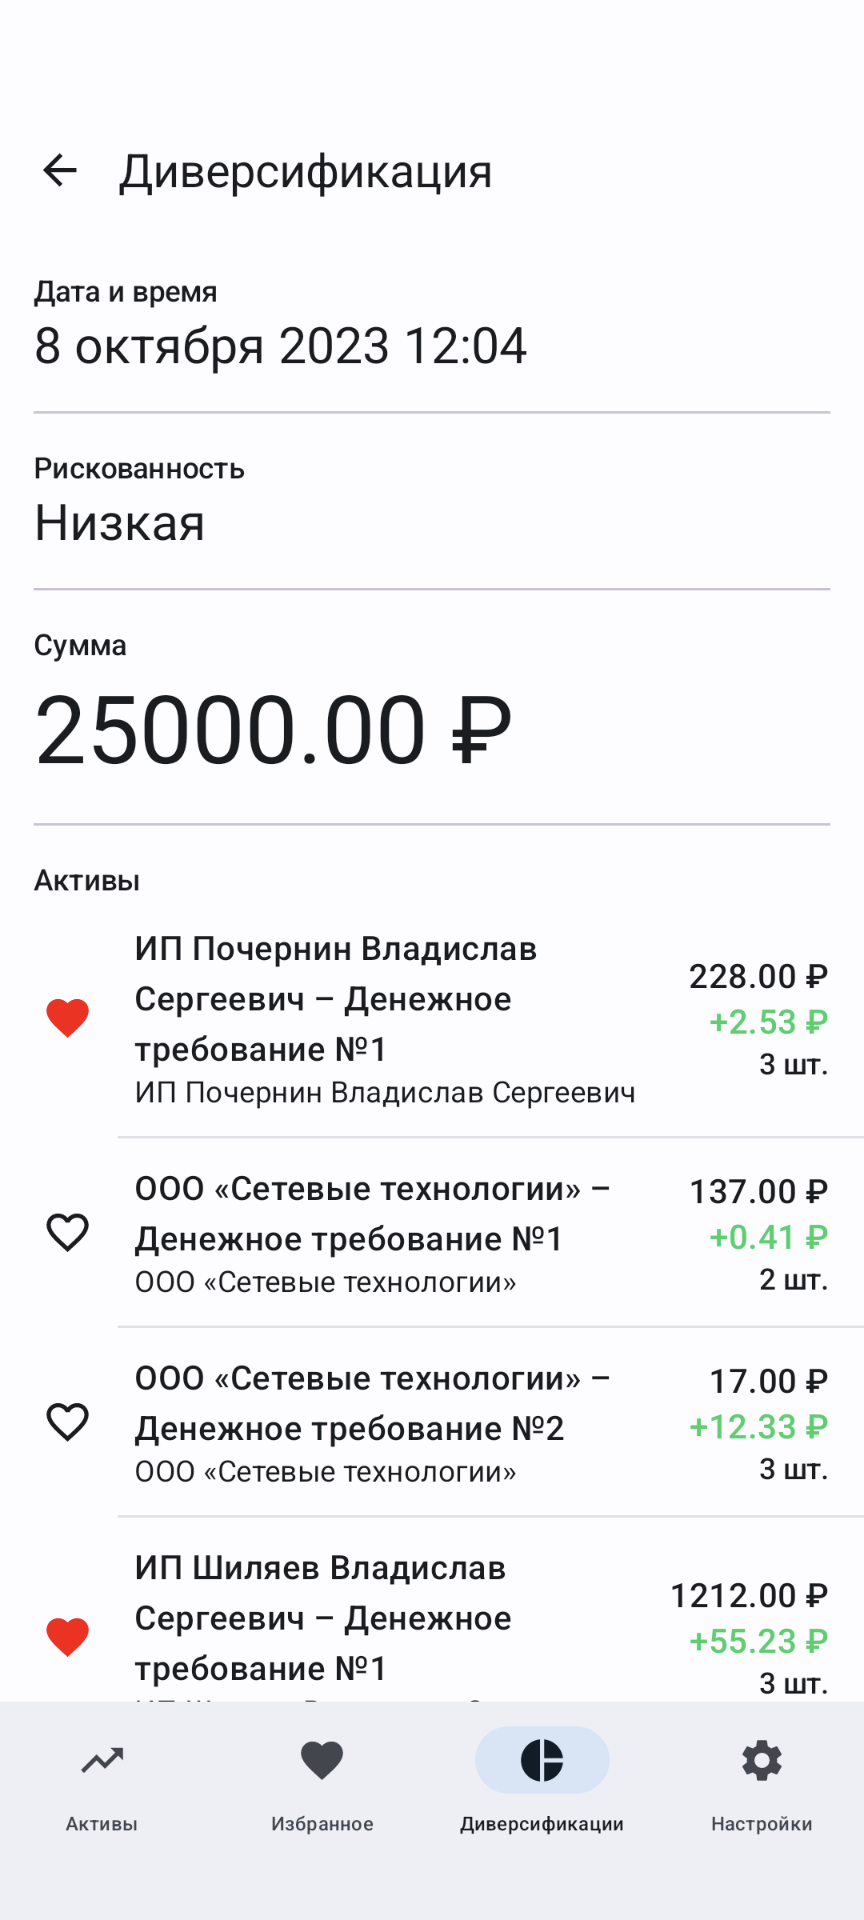
\includegraphics[width=5cm]{resources/12.png}
    \caption{Страница конкретной диверсификации (DiversificationPage)}
\end{figure}

\begin{figure}[H]
    \centering
    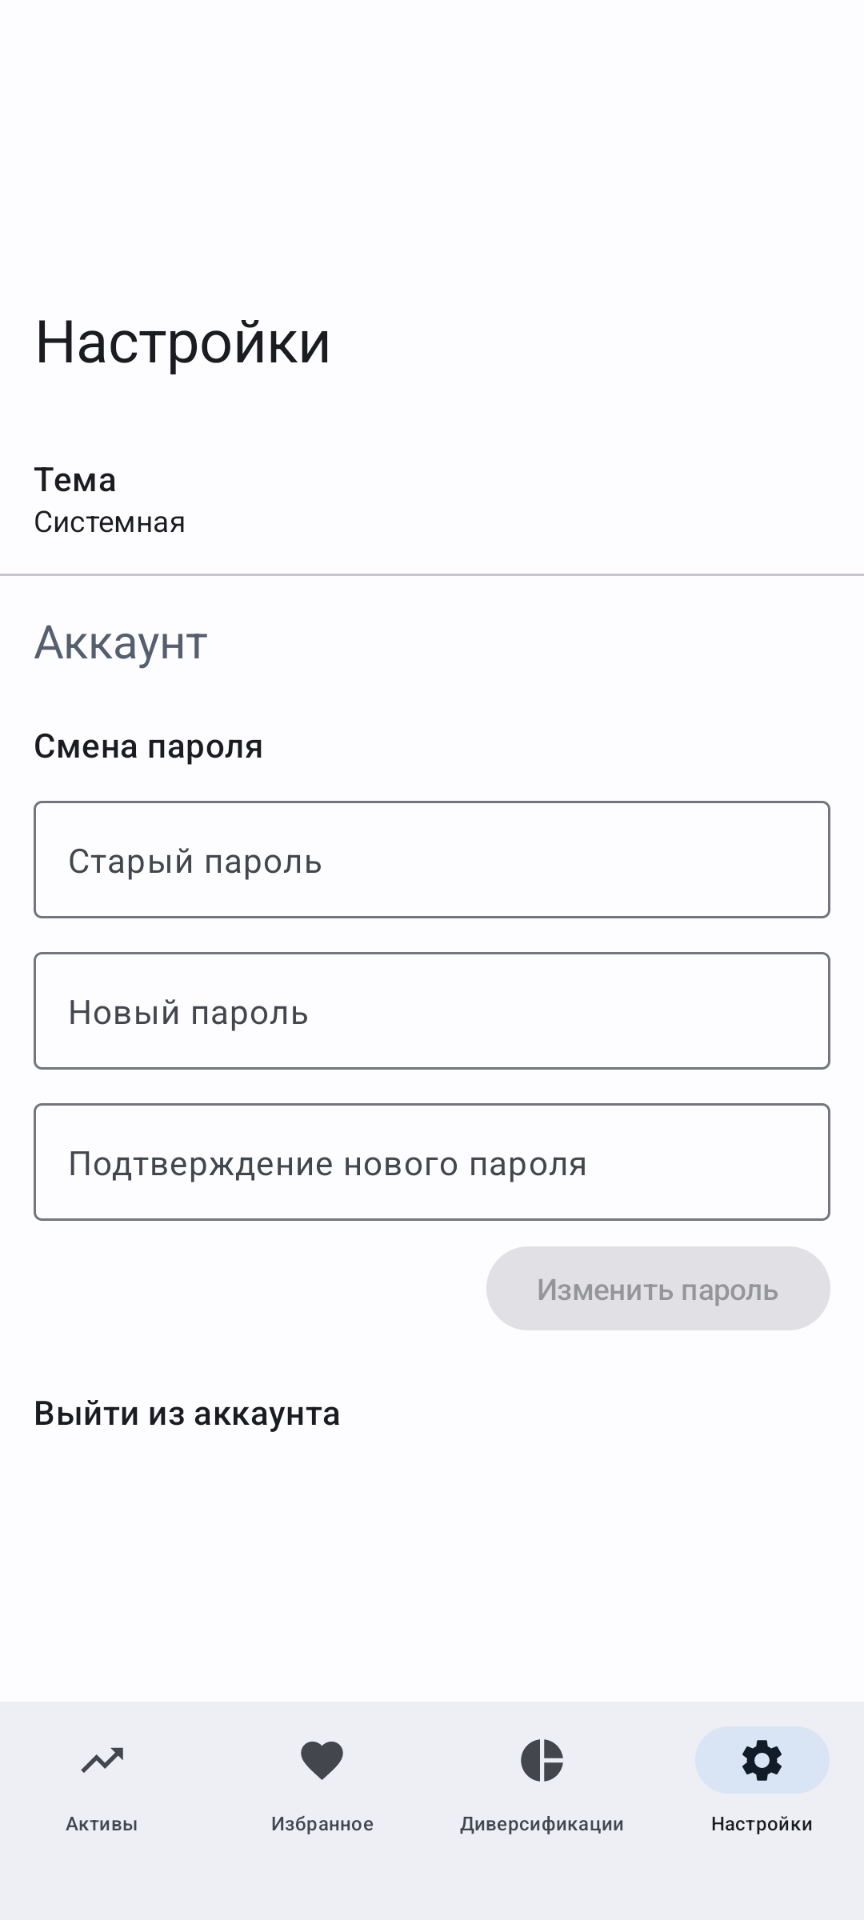
\includegraphics[width=5cm]{resources/13.png}
    \caption{Страница настроек (SettingsPage)}
\end{figure}

\end{document}